\chapter{Experiment and Evaluation}
\graphicspath{{Chapter5/Figs/}}

\begin{chapabstract}
Firstly, we introduce the dataset used for training and evaluating in our experiments. We also present the evaluation metrics and explain the reason for choosing those criteria. Then, the experiment results are shown in comparing to other proposed models. Finally, we present how to set up the environments for experiments.
\end{chapabstract}

\section{Dataset}
\label{sec:dataset}

In our experiment, we use 600,000 labeled training samples and 200,000 testing samples from Endgame Malware BEnchmark for Research (EMBER) dataset \cite{anderson2018ember}.

\begin{figure}[H] 
\centering
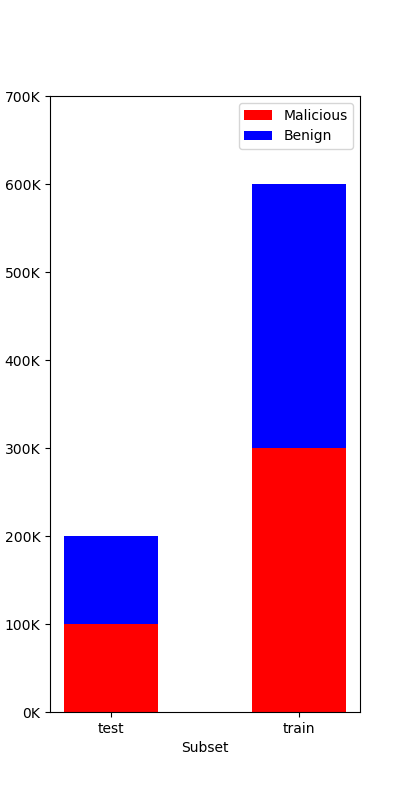
\includegraphics[width=0.5\textwidth]{dataset.png}
\caption{Distribution of samples in the dataset.}
\label{fig:ember}
\end{figure}
 
The EMBER dataset is the sizeable public dataset for malware detection which must include benign files and have an ideal ratio of malicious and benign files for machine learning tasks. This will solve the common problem of predictive accuracy, i.e., it will be misleading when the data is imbalanced. 

\section{Evaluation Criteria}

As discussed in section \ref{sec:objectives}, the goal of the thesis is to find a machine learning-based malware detection method that operates at a low false positive rate while tries to achieve a high detection rate.

\subsection{False Alarm Rate}

False positives, or false alarms, happen when a detector mistakes a malicious label for a benign file. We intend to make the false positive rate as low as possible, which is untypical for machine learning application. It is important because even one false alarm in a thousand benign files can create severe consequences for users. This problem is complicated by the fact that there are lots of clean files in the world, they keep appearing, and it is more challenging to collect these files. We evaluate the accuracy of our method at two specific false alarm rate values: at less than 0.1\%, and at less than 1\%.

\begin{center}
    ${False\ alarm\ rate} =  \cfrac{\sum False\ positive}{\sum Condition\ negative}$
\end{center}

\subsection{Detection Rate}

The detection rate, (eqv. with recall or true positive rate), measures the ratio of malicious programs detected out of the malware files used for testing. With higher recall, fewer actual cases of malware go undetected. In other words, the true positive rate shows the potential of how unseen binaries that were detected.

\begin{center}
    ${Detection\ rate} =  \cfrac{\sum True\ positive}{\sum Condition\ positive}$
\end{center}

\subsection{Area Under the ROC curve}

As introduced in section \ref{ssec:auroc}, the Area Under the ROC curve, AUROC or AUC for short, provides an aggregate measure of performance across all possible classification thresholds. AUC is scale-invariant and measures how well predictions are ranked, rather than their absolute values. Besides, AUC is classification-threshold-invariant, so that it can measure the quality of the predictions irrespective of what threshold is chosen. A model whose predictions are 100\% wrong has an AUC of 0.0, and the one whose predictions are 100\% correct has an AUC of 1.0.

A rough guide for classifying the accuracy of a classification test is the typical academic point system: 

\begin{itemize}
\item 0.9 - 1.0 = Excellent
\item 0.8 - 0.9 = Good
\item 0.7 - 0.8 = Fair
\item 0.6 - 0.7 = Poor
\item 0.5 - 0.6 = Fail
\end{itemize}

\section{Experimental Results}

The proposed GBDT-based malware detection method is implemented with LightGBM framework \cite{ke2017lightgbm}, and the input feature vectors have dimension of 1711. All our experiments were run on an instance which has 24 vCPUs and 32 GB memory. Using parallel programming, it took about 10 minutes to vectorize the raw features and about 5 minutes to train the model. The ROC curve of the final model is shown in Figure \ref{fig:roc_curve_with_highlights} and the distribution of scores for testing samples is shown in Figure \ref{fig:score_dist}.

\begin{figure}[H]
\centering
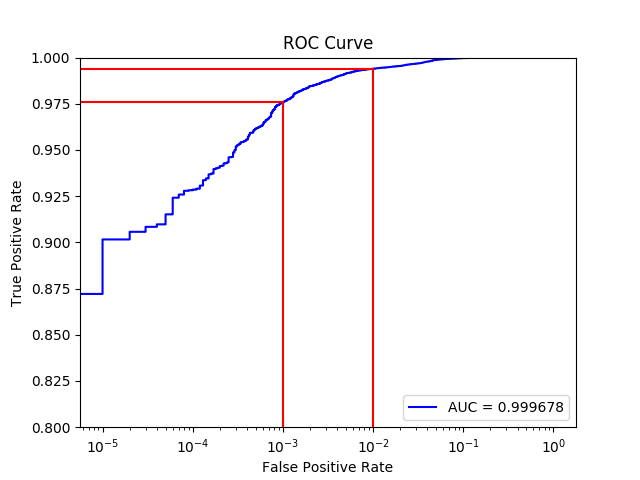
\includegraphics[width=\textwidth]{roc_curve_with_highlights.png}
\caption{The ROC curve of proposed model}
\label{fig:roc_curve_with_highlights}
\end{figure}

\begin{figure}[H] 
\centering
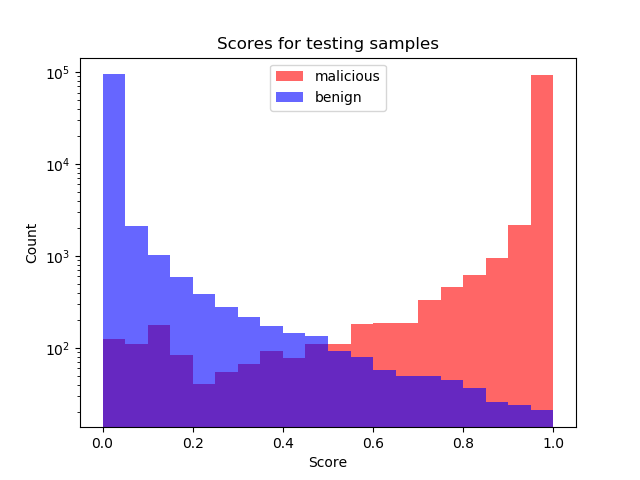
\includegraphics[width=\textwidth]{score_dist.png}
\caption{The distribution of scores for testing samples}
\label{fig:score_dist}
\end{figure}

The area under ROC curve exceeds $0.999678$, which means that almost all the predictions are correct. With a threshold of $0.828987$, the model score results in less than $0.1\%$ false alarm rate at a detection rate $97.5720\%$. At less than $1\%$ false positive rate, the model exceeds $99.3940\%$ detection rate with a threshold of $0.307897$. 

The baseline model has only the area under the ROC curve of $0.99911$, score results in less than $0.1\%$ FPR at TPR exceeding $92.99\%$, and at less than $1\%$ FPR, it exceeds $98.2\%$ TPR. Our model has better performance because of hyper-parameter tuning, and it also takes less time for training as a result of reducing feature space. Evidently, the model has better performance than the MalConv model trained on the raw binaries \cite{anderson2018ember}, which has ROC AUC is $0.99821$, corresponding to a $92.2\%$ TPR at a FPR less than 0.1\%, and a 97.3\% TPR at a less than 1\% FPR. Table \ref{table:training-time} and Table \ref{table:results} show the training time and evaluation results of our proposed model in comparison with MalConv model and the dataset owners’ baseline model.

\begin{table}[H]
\caption{The training time of our proposed model in comparison with MalConv model and the dataset owners’ baseline model}
\centering
\label{table:training-time}
\begin{tabular}{l l l l}
\hline
Model & Input &  Specifications & Training time \\
\hline
MalConv & Raw binaries & \begin{tabular}[c]{@{}l@{}} 2 NVDIA TITAN X \\ (Pascal) GPUs \end{tabular}  & \begin{tabular}[c]{@{}l@{}}10 days\\ (25 hours/epoch)\end{tabular}  \\
EMBER & 2351-value vectors & \begin{tabular}[c]{@{}l@{}} 8 vCPUs \\ (2015 MacBook Pro i7)\end{tabular}  & 20 hours \\ 
Our model & \textbf{1711}-value vectors & \begin{tabular}[c]{@{}l@{}} 24 vCPUs \\ (Google Compute Engine) \end{tabular}  & \textbf{10 minutes }\\ 
\hline 
\end{tabular}
\end{table}

\begin{table}[H]
\caption{The evaluation results of our proposed model in comparison with MalConv model and the dataset owners’ baseline model}
\centering
\label{table:results}
\begin{tabular}{l c c c}
\hline
Model                      & \begin{tabular}[c]{@{}c@{}}False Alarm Rate\\ (FPR)\end{tabular} & \begin{tabular}[c]{@{}c@{}}Detection Rate\\ (TPR)\end{tabular} & \begin{tabular}[c]{@{}c@{}}Area Under\\ the ROC curve (AUC)\end{tabular} \\

\hline
\multirow{2}{*}{MalConv}   & 0.1 \%                 & 92.200 \%            & \multirow{2}{*}{0.998210}                                                 \\
                           & 1.0 \%                 & 97.300 \%            &                                                                           \\
\multirow{2}{*}{EMBER}     & 0.1 \%                 & 92.990 \%            & \multirow{2}{*}{0.999110}                                                 \\
                           & 1.0 \%                 & 98.200 \%            &                                                                           \\
\multirow{2}{*}{Our model} & 0.1 \%                 & 97.572 \%            & \multirow{2}{*}{0.999678}                                                 \\
                           & 1.0 \%                 & 99.394 \%            &                                                                          
\\
\hline 
\end{tabular}
\end{table}

\section{Environment Setup Guide} 
\label{sec:research-env}

We mainly use the cross-platform tools in research and development for easily switching between operating systems. We use a Windows 10 Pro virtual machine for static malware analysis, an Ubuntu 16.04 LTS cloud instance for training and testing machine learning models, and use PyCharm Professional as mainly Integrated development environment (IDE).

\subsection{Windows environment for static analysis}

We use a virtual machine to build a background about malware:

\begin{itemize}
\item OS: Microsoft Windows 10 Pro
\item Version: 10.0.17134
\item Architecture: 64-bit
\end{itemize}

With following tools, we can easily gather malware basic information:

\begin{itemize}
 \item \textbf{CFF Explorer}: PE header parser.
 \item \textbf{PE Explorer} (from Heaventools Software): PE inspection tool.
 \item \textbf{BinText} (from McAfee): extract string from a binary.
 \item \textbf{HxD Hex Editor}: support for viewing file in binary format.
\end{itemize}

\subsection{Ubuntu environment for machine learning tasks}

\subsubsection{Google Cloud Platform}

We use an virtual machine for research, that can be deployed with the image from \textit{\href{https://console.cloud.google.com/launcher/details/ubuntu-os-cloud/ubuntu-xenial}{Cloud Launcher - Canonical - Ubuntu Xenial}}. The cloud instance has 24 virtual CPUs, 32 GB for memory, and is located in \verb|asia-southeast1-b| zone, i.e., Jurong West, Singapore.

After deployment, we add two optional firewall rules (\textit{\href{https://console.cloud.google.com/networking/firewalls/add}{VPC network - Firewall rules - Create a firewall rule}}), which allows all in and out connections for the virtual machine, to use Python Interactive Console features in PyCharm IDE.

\subsubsection{Anaconda}

We choose Anaconda, a free and open source distribution of the Python, to manage package and deploy. The content of \verb|environment.yml| used to deploy is shown below. 

\begin{lstlisting}
name: lab
channels:
  - conda-forge
dependencies:
  - python==3.6
  - matplotlib
  - numpy
  - scikit-learn
  - pip:
    - lief
    - git+https://github.com/onnx/onnxmltools
    - lightgbm
\end{lstlisting}

The environment is created with \textbf{Python 3.6} and packages for machine learning:

\begin{itemize}
\item \textbf{NumPy}: the fundamental package for scientific computing with Python.
\item \textbf{Matplotlib}: a Python 2D plotting library.
\item \textbf{Scikit-learn}: a machine learning library.
\item \textbf{Lief}: library to instrument executable formats.
\item \textbf{LightGBM}: a gradient boosting framework based on decision tree algorithms.
\item \textbf{ONNXMLTools}: a tool to convert models to ONNX format.
\end{itemize}

\subsection{PyCharm Professional IDE}

JetBrains provides \textit{\href{https://www.jetbrains.com/student/}{free individual licenses for students}} to use PyCharm Professional IDE. This is the powerful Python IDE, which gives us remote development capabilities and supports many scientific tools (e.g., Anaconda, Matplotlib and NumPy).

Following the guide \textit{\href{https://www.jetbrains.com/help/pycharm/configuring-remote-interpreters-via-ssh.html}{Configuring Remote Interpreters via SSH}} published by JetBrains, we can run, debug remotely from a cloud instance, which gives a great performance and is easy to scale.
